\section{Environment}
\subsection{Vim}
\textbf{vimrc}
\begin{lstlisting}[language=bash]
filetype indent on
syntax on

set nu
set cin
set sw=4
set sts=4
set ts=4
set so=99
set bs=2
set et
set hls

nn <c-j> :w <bar> :!g % <cr>

:au BufNewFile *.cpp r ~/.vim/main.cpp | 0d

inoremap {<cr> {<cr>}<esc>O

nn <silent> <space> :nohls <bar> :echo <cr>
\end{lstlisting} 
    
\textbf{template}    
\begin{lstlisting}[language=bash]
mkdir ~/.vim && vim ~/.vim/main.cpp  
\end{lstlisting} 

\textbf{bash} 
\begin{lstlisting}[language=bash]
export PATH=~/bin:$PATH
mkdir ~/bin/ && vim ~/bin/g
\end{lstlisting} 

\begin{lstlisting}[language=bash]
g++ -Wall -Wextra -std=c++14 -O2 -DLOCAL $1 -o exec || exit 1
echo Run
./exec || exit 1
echo Out
tail -20 *.out
\end{lstlisting} 

\begin{lstlisting}[language=bash]
chmod +x ~/bin/g
\end{lstlisting} 
\subsection{Clion}
\begin{itemize}

    \item Create \textbf{template} directory, add \textbf{main.cpp} with template code

    \item \textbf{init.sh}:
\begin{lstlisting}[language=bash]
for T in {A..L}; do
    mkdir -p $T
    cp -r template/. $T
    printf "set(CMAKE_RUNTIME_OUTPUT_DIRECTORY \${CMAKE_CURRENT_SOURCE_DIR}/$T)\n" >> CMakeLists.txt
    printf "add_executable($T $T/main.cpp)\n\n" >> CMakeLists.txt
done
\end{lstlisting}

\item Add this to \textbf{CMakeLists.txt}:
\begin{lstlisting}[language=bash]
set(CMAKE_CXX_STANDARD 14)
set(CMAKE_CXX_FLAGS "${CMAKE_CXX_FLAGS} -DLOCAL -Wall -Wextra -O2")
\end{lstlisting}

\item Settings $\to$ Editor $\to$ File Types $\to$ Ignore files and folder $\to$ add \textit{cmake-build-*}

\end{itemize}
\subsection{template.cpp}
\raggedbottom\lstinputlisting[style=cpp]{tmp/____env_code_templates_template.cpp}
\hrulefill
\subsection{template.java}
\raggedbottom\lstinputlisting[style=java]{tmp/____env_code_templates_template.java}
\hrulefill
\subsection{template.py}
\raggedbottom\lstinputlisting[style=py]{tmp/____env_code_templates_template.py}
\hrulefill

\section{Array transforms}
\subsection{hadamard}
\raggedbottom\lstinputlisting[style=cpp]{tmp/__array_transforms_hadamard.cpp}
\hrulefill
\subsection{fast subset convolution}
\raggedbottom\lstinputlisting[style=cpp]{tmp/__array_transforms_fast_subset_convolution.cpp}
\hrulefill
\subsection{fft doubles}
\raggedbottom\lstinputlisting[style=cpp]{tmp/__array_transforms_fft.cpp}
\hrulefill
\subsection{fft modulo}
\raggedbottom\lstinputlisting[style=cpp]{tmp/__array_transforms_mod_fft.cpp}
\hrulefill

\section{Strings}
\subsection{Fast lcs}
\raggedbottom\lstinputlisting[style=cpp]{tmp/__strings_fast_lcs.cpp}
\hrulefill
\subsection{Palindromic tree}
\raggedbottom\lstinputlisting[style=cpp]{tmp/__strings_palindromic_tree.cpp}
\hrulefill
\subsection{Suffix automaton}
\raggedbottom\lstinputlisting[style=cpp]{tmp/__strings_automaton.cpp}
\hrulefill
\subsection{Suffix array}
\raggedbottom\lstinputlisting[style=cpp]{tmp/__strings_suffix_array.cpp}
\hrulefill
\subsection{Manacher's algorithm}
\raggedbottom\lstinputlisting[style=cpp]{tmp/__strings_manacher.cpp}
\hrulefill

\section{Graphs}
\subsection{Dominator tree}
\raggedbottom\lstinputlisting[style=cpp]{tmp/__graphs_dominator_tree.cpp}
\hrulefill
\subsection{Kuhn / 32}
\raggedbottom\lstinputlisting[style=cpp]{tmp/__graphs_kuhn_div32.cpp}
\hrulefill
\subsection{Two chinese}
\raggedbottom\lstinputlisting[style=cpp]{tmp/__graphs_two_chinese.cpp}
\hrulefill
\subsection{Weighted matroid intersection}
\raggedbottom\lstinputlisting[style=cpp]{tmp/__graphs_weighted_matroid_intersection.cpp}
\hrulefill
\subsection{Weighted kuhn}
\raggedbottom\lstinputlisting[style=cpp]{tmp/__graphs_weighted_kuhn.cpp}
\hrulefill
\subsection{Fast dinic}
\raggedbottom\lstinputlisting[style=cpp]{tmp/__graphs_dinic.cpp}
\hrulefill

\section{Geometry}
\subsection{General templates}
\raggedbottom\lstinputlisting[style=txt]{tmp/__geometry_geometry.h}
\hrulefill
\subsection{Convex hull}
\raggedbottom\lstinputlisting[style=cpp]{tmp/__geometry_convex_hull.cpp}
\hrulefill
\subsection{Halfplanes intersection}
\raggedbottom\lstinputlisting[style=cpp]{tmp/__geometry_halfplanes_intersection.cpp}
\hrulefill

\section{Number theory}
\subsection{Integer points under line}
\raggedbottom\lstinputlisting[style=cpp]{tmp/__number_theory_under_line.cpp}
\hrulefill
\subsection{Chinese remainder theorem}
\raggedbottom\lstinputlisting[style=cpp]{tmp/__number_theory_crt.cpp}
\hrulefill

\section{Algebra}
\subsection{Gauss}
\raggedbottom\lstinputlisting[style=cpp]{tmp/__algebra_gauss.cpp}
\hrulefill

\section{Notes}
\subsection{Bugs}
\begin{itemize}
    \item \foreignlanguage{russian}{Общее}
        \begin{enumerate}
            \item \foreignlanguage{russian}{В задаче просят выводить массив int-ов посортированным, а я это не делаю.}
            
            \item \foreignlanguage{russian}{Бесконечность = максимальному возможному числу
(когда это приводит к нежелательному результату).}

            \item \foreignlanguage{russian}{НЕправильно: v.resize(q); forn (i, q) v.pb(...)\\ правильно: v.resize(q); forn (i, q) v[i] = ...}

            \item \foreignlanguage{russian}{Аккуратнее с глобальными переменными. В частности, не использовать общий used
при рекурсивном подсчёте чисел Гранди в стиле
tmr++; for (int x : sons) used[grundy(x)] = tmr;
(проблема в том, что used-ы могут перезаписаться, когда мы пойдём в ребёнка).}

        \end{enumerate}

    \item \foreignlanguage{russian}{Геометрия} 
        \begin{enumerate}
            \item \foreignlanguage{russian}{Когда смотришь, на какой угол надо повернуть прямую, чтобы она пересекла
            многоугольник, получается на самом деле два отрезка углов (так как поворот прямой
                на a in [0, pi) и a + pi есть одно и то же).}
            \item \foreignlanguage{russian}{Не писать проверку принадлежности точки многоугольники
            с площадями в случае даблов (хреново с точностью для точек около
            границы). Правильно с суммой углов.}
        \end{enumerate}

\end{itemize}

\subsection{Ideas}
\begin{itemize}
    \item 
\foreignlanguage{russian}{[CF 381 Div 1 E] Пусть есть динамика $dp[n][a][b]$ за $O(n^3)$, где мы как-то делаем O(1)
переходов вида добавить значение c за x b-шек, y a-шек. Если при этом оптимальный ответ
всегда в $dp[n][a][b]$, то можно вместо $dp[n][a][b]$ хранить $dp[n][a][b] - c \cdot b$. Это ещё
ничего не даёт само по себе, но позволяеет написать динамику dp[n][a], cnt[n][a] -
подвинутое значение динамики, которого мы добились, а cnt - число использованных при
этом b-шек. Теперь заметим, что большие $c$ заставляют нас избегать b-шек и их используется
больше $b$. Сильно отрицательные заставляют нас набирать b-шки со страшной силой. Нам нужно
найти в точности ту границу, где $cnt[n][a] = b$ и посчитать там.}

\item
\foreignlanguage{russian}{[Задача Tree Embedding с какого-то китайского контеста в Петрозаводске] Естественную
метрику на дереве (расстояние между вершинами есть число рёбер между ними) с n вершинами
можно смоделировать с помошью $l_{\infty}^{O(\log{n})}$ (то есть вектора с $O(\log{n})$ координатами,
что $d(x, y) = max_i |x_i - y_i|$). Ссылка на алгоритм в комментариях
к} http://codeforces.com/blog/entry/49117.

\item
\foreignlanguage{russian}{
[Hackerrank 101 Hack 43, часть задачи E]
Посчитать число способов представить k как сумму различных слагаемых от 1 до $n$ за $O(k^{\frac{3}{2}})$.
Cчитаем динамику $dp[cnt][sum]$ - число способов набрать sum с помощью cnt элементов
(не имеет смысл использовать $cnt$ больше $O(\sqrt{k})$. Считаем так: $dp[i][j] =
dp[i - 1][j - i] + dp[i][j - i] - dp[i - 1][j - n - 1]$ (уменьшим все слагаемые на один, их
осталось либо снова $i$, либо $i - 1$ (ушла единица), при этом посчитали лишние состояния,
где в сумму после уменьшения входило $n$ (а значит в текущую сумму входит $n+1$, что запрещено),
их ровно столько, сколько нормальных состояний с $i - 1$ элементом и суммой $j - n - 1$.
Аналогично, если надо посчитать со знаком $(-1)^{|S|}$. Код для этого случая (со знаком):}
\begin{lstlisting}[language=c++]
forn (i, L + 1) forn (j, k + 1) if (dp[i][j])
{
	add(res[j], dp[i][j]);
	if (i + 1 <= L && j + i + 1 <= k)
		sub(dp[i + 1][j + i + 1], dp[i][j]);
	if (j + i <= k) if (i)
		add(dp[i][j + i], dp[i][j]);
	if (j + n + 1 <= k && i + 1 <= L)
		add(dp[i + 1][j + n + 1], dp[i][j]);
}
\end{lstlisting}

\item
\foreignlanguage{russian}{Число перестановок $n$ элементов
с ровно $k$ инверсиями есть коэффициент при $x^k$ многочлена \\
$(1 + x + x^2 + \ldots + x^{n - 1})(1 + x + x^2 + \ldots + x^{n - 2}) \ldots (1 + x) \cdot 1$ \\
(смотрим на
тупую динамику и радуемся), что есть \\
$(1 - x)^{-n} (1 - x) (1 - x^2) \ldots (1 - x^n)$. \\
Если
$k \leq n$, то можно заменить на \\
$(1 - x)^{-n} \prod\limits_{i = 1}^{+\infty} (1 - x^i) = (1 - x)^{-n} \sum\limits_{q = -\infty}^{+\infty} (-1)^q \cdot x^{3q(q + 1)/2}$ \\
(пентагональная
теорема Эйлера).}

\item
\foreignlanguage{russian}{[Задача с контеста СГУ в ПТЗ зима 2016 про три сервера, задача про покемонов
(см. пост krismaz на CF]. Пусть надо выбрать ровно $k$ объектов из $n$ и есть
какая-то динамика типа $dp[x][y]$ - выбрали ровно $y$ объектов из первых $x$.
(возвращаем $dp[n][k]$). Можно предварительно пошаффлить объекты и тогда
нет смысла рассматривать состояния $dp[x][y]$ с слишком большим
$|y - \frac{xk}{n}|$, так как теперь объекты из оптимального решения распределены
случайно (отклоняемся на $O(\sqrt{n})$).}

\item
\foreignlanguage{russian}{[Opencup GP of Poland 2017, задача A]. Если нужно посчитать число строк, не содержащих
данных в качестве подстрок на фиксированных позиций (похоже на Ахо-Корасик, но не
совсем то же самое), то можно это делать персистентным бором.}

\item
\foreignlanguage{russian}{[Птз-лето 2017, восьмой день, Convex polygons (задача G)]\\
Можно считать $\sum\limits_{y=l}^r p(y) {y \choose x}$, где $p$ - многочлен, разложив
$p$ по базису $1$, $t$, $t(t+1)/2$, $t(t+1)(t+2)/6$, $\ldots$ Например, \\
$\sum\limits_{y=1}^r y \cdot {y \choose x} = \sum\limits_{z=1}^r \sum\limits_{y=z}^r {y \choose x} =
\sum\limits_{z=1}^r ({r+1 \choose x} - {z+1 \choose x})$ и так далее (свернуть ещё раз).}\\
Hockey stick theorem: $\sum\limits_{y=x}^{r} {y \choose x} = {r+1 \choose x+1}$

\item
\foreignlanguage{russian}{Пусть есть некоторая динамика с циклическими зависимостями
(обычно матожидание какого-то времени), которая тем не менее однозначно
выражается через одно из своих значений. Тогда очень часто работает такой
трюк: сделать бинпоиск по этому значению X, а потом поcчитать его по-нормальному,
заменяя все его вызовы на X (и получить Y). Если X < Y, то X меньше ответа,
если X > Y, то X больше ответа.}

\end{itemize}

\subsection{Info}
\begin{itemize}
	\item A lot of divisors
	\begin{itemize}
		\item $\leq 20: d(12)=6$
		\item $\leq 50: d(48)=10$
		\item $\leq 100: d(60)=12$
		\item $\leq 1000: d(840)=32$
		\item $\leq 10^4: d(9240)=64$
		\item $\leq 10^5: d(83160)=128$
		\item $\leq 10^6: d(720720)=240$
		\item $\leq 10^7: d(8648640)=448$
		\item $\leq 10^8: d(91891800)=768$
		\item $\leq 10^9: d(931170240)=1344$
		\item $\leq 10^{11}: d(97772875200)=4032$
		\item $\leq 10^{12}: d(963761198400)=6720$
		\item $\leq 10^{15}: d(866421317361600)=26880$
		\item $\leq 10^{18}: d(897612484786617600)=103680$
	\end{itemize}

	\item Numeric integration
	\begin{itemize}
		\item simple: $F(0)$
		\item simpson: $\frac{F(-1) + 4 \cdot F(0) + F(1)}{6}$
		\item runge2: $\frac{ F(-\sqrt{\frac{1}{3}}) + F(\sqrt{\frac{1}{3}}) }{2}$
		\item runge3: $\frac{ F(-\sqrt{\frac{3}{5}}) \cdot 5 + F(0) \cdot 8 +  F(\sqrt{\frac{3}{5}}) \cdot 5}{18}$
	\end{itemize}
\end{itemize}	

\section{Images}
\subsection{Hex}
\pagebreak
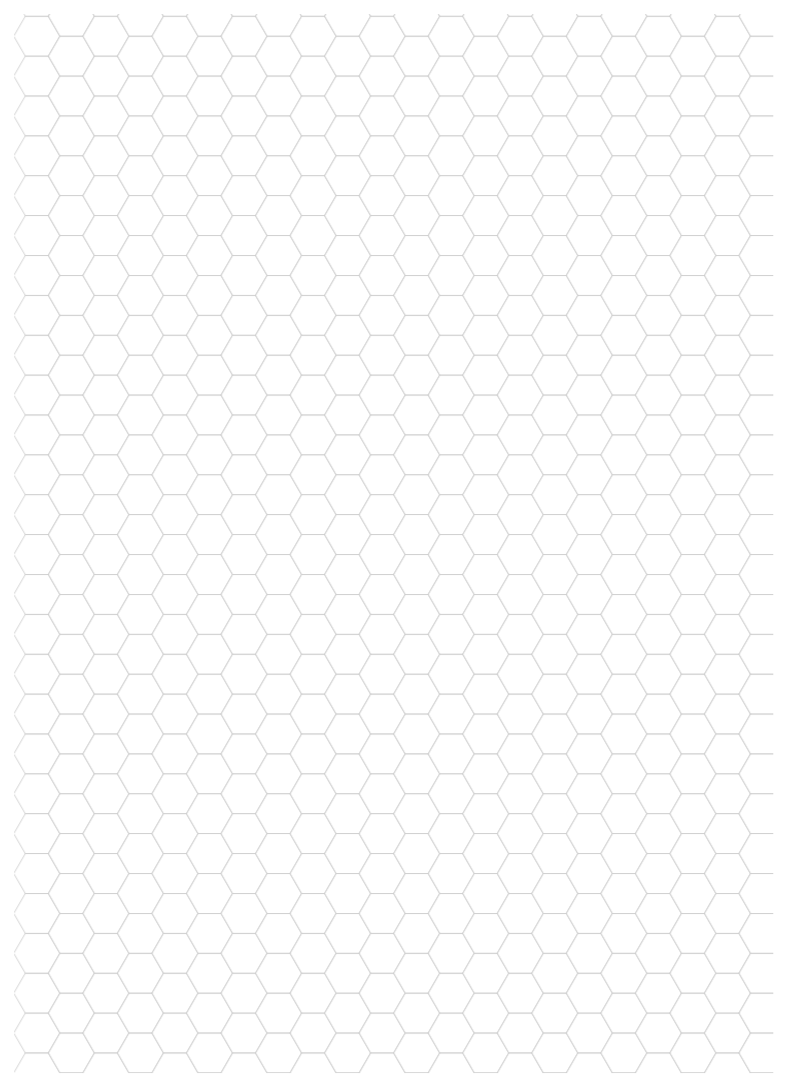
\includegraphics[scale=1.3]{hex3.png}
